%%
%% Author: thompson
%% 04.11.17
%% THIS FUCKING LANGUAGE

% Preamble
\documentclass[11pt]{article}

% Packages
\usepackage{a4wide}

\usepackage{verbatim}
\usepackage{graphicx}

% Document
\begin{document}
    \section{Some combined hate on \texttt{Javascript}}

    \subsection{RegEx}
    Regex in .js are the same as goddamn ploughin anywhere, but the implementation of
    this greasy-bottom muffPutter kinda differs from the usual Java.

    \begin{verbatim}
        - regexObject.test( String )
        Executes the search for a match between a regular expression
         and a specified string.
        Returns true or false.

        - string.match( RegExp )
        Used to retrieve the matches when matching a string against
         a regular expression.
        Returns an array with the matches or null if there are none.
         and null evaluates to false.
    \end{verbatim}

    Performance-Wise, use .test().\\
    \begin{center}
        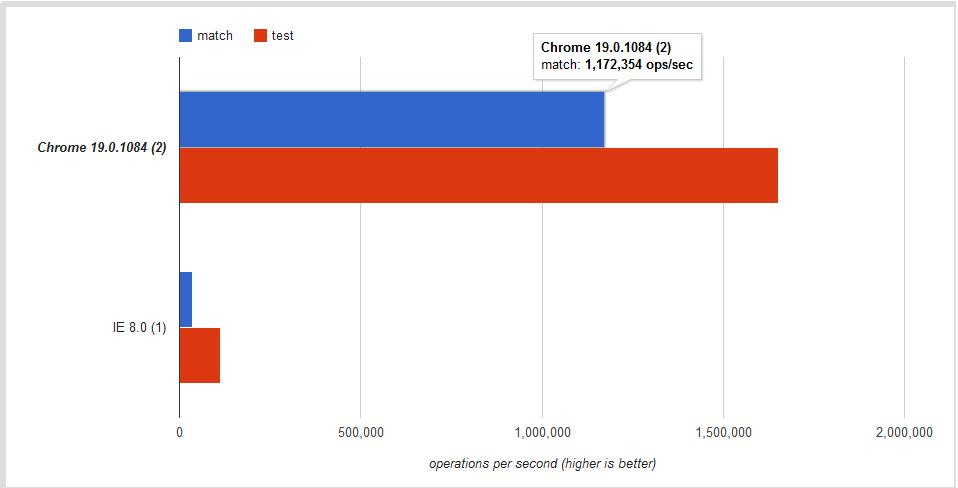
\includegraphics[width=\textwidth]{jsRegex.jpg}
    \end{center}

    \subsection{Calling Functions}
    There is no 'get-over-here by Reference', unless objectified like women.
    \begin{verbatim}
        function passVar(obj1, obj2, num) {
        obj1.prop = "laptop";           // will CHANGE original
        obj2 = { prop: "computer" };    //will NOT affect original
        num = num + 1;                  // will NOT affect original
        }

        var object1 = {
        prop: "car"
        };
        var object2 = {
        prop: "bike"
        };
        var number1 = 10;

        passVar(object1, object2, number1);
        console.log(object1); //output: Object {item:"laptop"}
        console.log(object2); //output: Object {item:"bike"}
        console.log(number1); //ouput: 10
    \end{verbatim}
\end{document}